\documentclass[11pt,a4paper]{book}
\usepackage[utf8]{inputenc}
\usepackage[OT1]{fontenc}
\usepackage[english]{babel}
\usepackage{amsmath}
\usepackage{amsfonts}
\usepackage{amssymb}
\usepackage{graphicx}


% Tikz to draw blocky diagrams
\usepackage{tikz}
\usetikzlibrary{shapes,arrows,chains,calc,positioning,fit}

	% We need layers to draw the block diagram
\pgfdeclarelayer{background}
\pgfdeclarelayer{foreground}
\pgfsetlayers{background,main,foreground}

\begin{document}	


	
\chapter{Notes}

\section{ReferencableChunk}
A chosen name for an abstract block of data within a RevisionStoreFile according to MS-ONESTORE.
To parse the document there are 4 structures which reference file locations by an absolute position.
If we want to change the size of a chunk within the file, all chunks which follow the changed-size chunk will be not referenced correctly anymore.
That’s why we need a structure which records the file structure and is able to calculate the stream pointer value as dependent from that structure.
Each referencable chunk has the property of being serially parsed without the need to jump to an other file location.

The following objects have been identified to qualify as such referencable chunk:
\begin{itemize}
\item RevisionStoreFileHeader
\item FileNodeListFragmentHeader*
\item FileNode
\item FileNodeListFooter*
\item FreeChunkListFragment
\item FreeChunk
\item TransactionLogFragment
\item FileDataStoreObject
\item ObjectSpaceObjectPropSet
\item ObjectInfoDependencyOverrideData
\item EncryptedFragment.
\end{itemize}
* The FileNodeListFragment containes a number of FileNodes. To avoid branching the FileNodeListFragment will be considered to consists of a FileNodeListFragmentHeader, FileNodeListFragmentFooter, as individual ReferencableChunk as well as FileNodes

\subsection{FreeChunkListFragment}

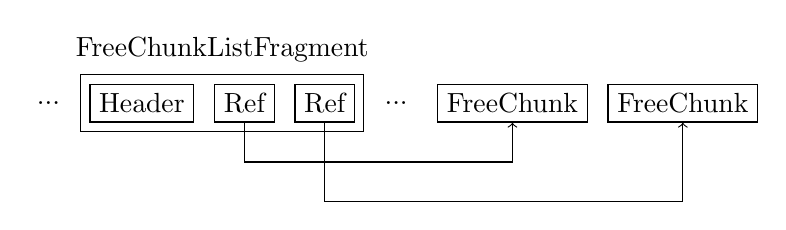
\begin{tikzpicture}[start chain=going right,node distance=0.25cm] 
	\node [on chain] {...};
			\node [draw, on chain] (header) {Header};
	\node [draw, on chain] (ref1) {Ref};
	\node [draw, on chain] (ref2) {Ref};
	
    \node [draw,fit={($(header.south west)+(.5*\pgflinewidth,0)$) 
	($(ref2.north east)-(.5*\pgflinewidth,0)$)}] (listfragment) {};
	\node [above=1pt of listfragment.north] {FreeChunkListFragment};
	
	\node [on chain] (more) {...};
	\node [draw, on chain] (freechunk1) {FreeChunk};
	\node [draw, on chain] (freechunk2) {FreeChunk};
	
	\draw[->] (ref1) -- ($(ref1.south) - (0,0.5cm)$) -- ($(freechunk1.south) - (0,0.5cm)$) ->(freechunk1);
	\draw[->] (ref2) -- ($(ref2.south) - (0,1cm)$) -- ($(freechunk2.south) - (0,1cm)$) ->(freechunk2);
\end{tikzpicture}
\end{document}





